%\documentclass[10pt,xcolor={dvipsnames},fleqn]{beamer}
\documentclass[handout,10pt,xcolor={dvipsnames},fleqn]{beamer}
\usepackage{isse}


\usepackage{apalike}
\usepackage[utf8]{inputenc}
\usepackage{pdfpages}
%\usepackage{ngerman}
\usepackage{stmaryrd,amsmath,amssymb}
\usepackage{color}
\usepackage{enumerate}
\usepackage[makeroom]{cancel}
\usepackage{mdframed}
\usepackage{xskak}
\usepackage{fancyvrb}
\usepackage{marvosym}
\setchessboard{
showmover=false}
\usepackage[noend]{algpseudocode}   % package for algorithms
\usepackage{algorithm}
\usepackage{tikz}

\usepackage[absolute,overlay]{textpos}

\usetikzlibrary{trees,calc,shapes,arrows,matrix,shadows,decorations.markings}
\usetikzlibrary{decorations.pathreplacing}
\usetikzlibrary{calc,shapes.callouts,shapes.arrows}
\usetikzlibrary{decorations.text}
\newcommand{\CustomCite}[1]{\color{issegrey} \textbf{#1}}
\tikzset{
   hierNode/.style={main node,text width=1.1em,text centered,inner sep=1pt},
   bStyle/.style={fill=forestgreen!35},
   cStyle/.style={fill=black!35},
   dStyle/.style={fill=thermicred!25},
   optboundaries/.style={
           state,
           rectangle,
           rounded corners,
           draw=black, thick,
           minimum height=4em,
           minimum width=7em,
           inner sep=2pt,
           text centered,
           dashed
           },
  trajectory/.style={issegrey,-},
  emph/.style={isseorange},
  trajectorynode/.style={fill=issegrey},
  hystate/.style={
           state,
           rectangle,
           rounded corners,
           draw=black, very thick,
           minimum height=1em,
           minimum width=2em,
           inner sep=1pt,
           text centered,
           },
 hystatel/.style={
 		   hystate, 
 		   inner sep=3pt
 }
}


\mdfdefinestyle{theoremstyle}{
linecolor=red,linewidth=2pt,
frametitlerule=true,
frametitlebackgroundcolor=gray!20,
innertopmargin=\topskip,
}
\definecolor{LRed}{rgb}{1,.8,.8}
\definecolor{MRed}{rgb}{1,.6,.6}
\definecolor{HRed}{rgb}{1,.2,.2}

\usepackage{listings}
\lstdefinelanguage{mzn}
{
	morekeywords={var,morph,pareto,lex,par,int,solve,not,search,satisfy,new,endif,maximize,params,instantiates,with,bool,in,type,PVS,PVSType,minimize,float,constraint,soft,sum,forall,exists,array,of,include,predicate,then,commit,post,set,function,if,else,repeat,next,ann,break},
	sensitive=false,
	morecomment=[l]{\%},
	morecomment=[s]{/*}{*/},
	morestring=[b]",
}


\definecolor{lightlightgray}{gray}{0.95}
\definecolor{forestgreen}{HTML}{009B55}
\definecolor{thermicred}{rgb}{0.82, 0.1, 0.26}
\lstset
{
	basicstyle=\ttfamily\small,
	commentstyle=\ttfamily\color{thermicred},
	stringstyle=\ttfamily\color{isseorange},
	keywordstyle=\ttfamily\color{blue},
	tabsize=2,
	showstringspaces=false,
	flexiblecolumns=true,
	captionpos=b,	
	backgroundcolor=\color{lightlightgray},
	frame=single,
	 xleftmargin=\parindent,
}

\lstset{language=mzn}
\interfootnotelinepenalty=10000

% ====== custom commands

\newcommand{\prosumer}[1]{\ensuremath{\mathtt{#1}}}
% Soft Constraint Example
\newcommand{\constraintName}[1]{\ensuremath{\mathtt{#1}}}
% Biogas Constraints
\newcommand{\biogas}{biogas}
\newcommand{\biogasShort}{bio}
\newcommand{\gasFull}{\ensuremath{\constraintName{gasFull}_\mathtt{\biogasShort}}}
\newcommand{\ecoSweet}{\ensuremath{\constraintName{ecoSweet}_\mathtt{\biogasShort}}}
\newcommand{\onOff}{\ensuremath{\constraintName{onOff}_\mathtt{\biogasShort}}}
% Thermal Plant Constraints
\newcommand{\thermal}{thermal}
\newcommand{\thermalShort}{therm}
\newcommand{\ecoOpt}{\ensuremath{\constraintName{ecoOpt}_\mathtt{\thermalShort}}}
\newcommand{\inertia}{\ensuremath{\constraintName{inertia}_\mathtt{\thermalShort}}}
\newcommand{\ecoGood}{\ensuremath{\constraintName{ecoGood}_\mathtt{\thermalShort}}}
\newcommand{\hLevelThermal}[1]{$H_#1^\mathtt{\thermalShort}$}
% Electric Vehicle
\newcommand{\ev}{EV}
\newcommand{\limitBatteryUsage}{\ensuremath{\constraintName{limitBU}_\mathtt{\ev}}}
\newcommand{\prefBatteryLevel}{\ensuremath{\constraintName{prefBL}_\mathtt{\ev}}}
\newcommand{\earlyBird}{\ensuremath{\constraintName{earlyBird}_\mathtt{\ev}}}
% Organization
\newcommand{\org}{org}
\newcommand{\minMaxViolation}{\ensuremath{\constraintName{violation}_\mathtt{\org}}}
\newcommand{\hLevelOrg}[1]{$H_#1^\mathtt{\org}$}

\newcommand{\Variable}{X}
\newcommand{\LocalVariable}{\widehat{\Variable}}
\newcommand{\Domain}{D}
\newcommand{\Constraint}{C}
\newcommand{\ConstraintRelationship}{\mathcal{R}}

\newcommand{\valuation}{v}
\newcommand{\constraint}[1]{\mathrm{#1}}

\newcommand{\plantconstraint}[3]{  
\ifx#1b \constraint{best}[#3]
\else \ifx#1g \constraint{good}[#3]
\else \ifx#1a \constraint{acc}[#3]
\else \ifx#1d \constraint{diff}
\else \ifx#1l \constraint{low}[#3]
\else \ifx#1h \constraint{high}[#3]
\else \ifx#1o \constraint{org}[#3]
   \else
   \constraint{#1}_{#2}^{#3} 
   
   
\fi \fi \fi \fi \fi \fi \fi}
\usepackage{stmaryrd}

\newcommand{\code}[1]{\normalfont\texttt{\spaceskip=3pt\frenchspacing\def\{{\char123}\def\}{\char125}\def\^{\char94}\def\_{\char95}#1}}
\newcommand{\varit}[1]{{\frenchspacing\ensuremath{\normalfont\textsl{#1}}}}
\newcommand{\macit}[1]{{\frenchspacing\ensuremath{\normalfont\textsf{#1}}}}
\newcommand{\Eta}{\mathrm{H}}
\newcommand{\Mu}{\mathrm{M}}
\newcommand{\Nu}{\mathrm{N}}

\newcommand{\NZ}{\mathbb{N}}
\newcommand{\RZ}{\mathbb{R}}
\newcommand{\RZp}{\RZ_{\geq 0}}
\newcommand{\powerset}{\mathcal{P}}
\newcommand{\limp}{\mathrel{\Rightarrow}}
\newcommand{\compfun}{\mathbin{\circ}}
\newcommand{\isorel}{\mathrel{\cong}}
\newcommand{\restrict}[2]{{#1}\mathnormal{\upharpoonright}{#2}}
\newcommand{\natto}{\mathrel{\dot{\mathnormal{\to}}}}
\let\lbagold\lbag
\let\rbagold\rbag
\def\lbag{\mathopen{\lbagold}}
\def\rbag{\mathclose{\rbagold}}

\DeclareMathOperator{\Minop}{\mathrm{Min}}
\newcommand{\Min}[1]{\Minop^{#1}}
\DeclareMathOperator{\Maxop}{\mathrm{Max}}
\newcommand{\Max}[1]{\Maxop^{#1}}
\DeclareMathOperator{\finsets}{\mathcal{P}_{\mathrm{fin}}}
\DeclareMathOperator{\nefinsets}{\mathcal{P}_{\mathrm{fin}^+}}
%\DeclareMathOperator{\incfinsets}{\mathcal{I}_{\mathrm{fin}}}
\newcommand{\incfinsets}[1]{\mathcal{I}_{\mathrm{fin}}^{#1}}
\newcommand{\lowersubseteq}[1]{\mathrel{\subseteq_{#1}}}
\newcommand{\lowersupseteq}[1]{\mathrel{\supseteq_{#1}}}
\newcommand{\lowersubset}[1]{\mathrel{\subset_{#1}}}
\newcommand{\lowersupset}[1]{\mathrel{\supset_{#1}}}
\newcommand{\uppersubseteq}[1]{\mathrel{\subseteq^{#1}}}
\newcommand{\uppersupseteq}[1]{\mathrel{\supseteq^{#1}}}
\newcommand{\uppersubset}[1]{\mathrel{\subset^{#1}}}
\newcommand{\uppersupset}[1]{\mathrel{\supset^{#1}}}
\newcommand{\lowercup}[1]{\mathbin{\cup_{#1}}}
\newcommand{\uppercup}[1]{\mathbin{\cup^{#1}}}

\DeclareMathOperator{\finmsets}{\mathcal{M}_{\mathrm{fin}}}
\DeclareMathOperator{\nefinmsets}{\mathcal{M}_{\mathrm{fin}^+}}
\newcommand{\mcup}{\mathbin{\mathnormal{\cup}\llap{\text{\fontsize{8pt}{8pt}\selectfont$-$}}}}
\newcommand{\submseteq}{%
\mathrel{\mathchoice%
{\mathnormal{\subseteq}\llap{\text{\raisebox{0.3pt}{\fontsize{8pt}{8pt}\selectfont\rotatebox{90}{$-$}\hspace{1.8pt}}}}}%
{\mathnormal{\subseteq}\llap{\text{\raisebox{0.3pt}{\fontsize{8pt}{8pt}\selectfont\rotatebox{90}{$-$}\hspace{1.8pt}}}}}%
{\mathnormal{\subseteq}\llap{\text{\raisebox{-0.3pt}{\fontsize{5pt}{5pt}\selectfont\rotatebox{90}{$-$}\hspace{1.4pt}}}}}%
{\mathnormal{\subseteq}\llap{\text{\raisebox{-0.3pt}{\fontsize{5pt}{5pt}\selectfont\rotatebox{90}{$-$}\hspace{1.4pt}}}}}%
}}
\newcommand{\supmseteq}{\mathrel{\reflectbox{$\submseteq$}}}
\newcommand{\lowersubmseteq}[1]{\mathrel{\submseteq_{#1}}}
\newcommand{\uppersubmseteq}[1]{\mathrel{\submseteq^{#1}}}
\newcommand{\submset}{%
\mathrel{\mathchoice%
{\mathnormal{\subset}\llap{\text{\raisebox{-0.8pt}{\fontsize{8pt}{8pt}\selectfont\rotatebox{90}{$-$}\hspace{1.8pt}}}}}%
{\mathnormal{\subset}\llap{\text{\raisebox{-0.8pt}{\fontsize{8pt}{8pt}\selectfont\rotatebox{90}{$-$}\hspace{1.8pt}}}}}%
{\mathnormal{\subset}\llap{\text{\raisebox{-0.3pt}{\fontsize{7pt}{7pt}\selectfont\rotatebox{90}{$-$}\hspace{1pt}}}}}%
{\mathnormal{\subset}\llap{\text{\raisebox{-0.3pt}{\fontsize{7pt}{7pt}\selectfont\rotatebox{90}{$-$}\hspace{1pt}}}}}%
}}
\newcommand{\supmset}{\mathrel{\reflectbox{$\submset$}}}
\newcommand{\lowersubmset}[1]{\mathrel{\submset_{#1}}}
\newcommand{\uppersubmset}[1]{\mathrel{\submset^{#1}}}

\DeclareMathOperator{\collapseset}{\mathcal{C}}

\newcommand{\category}[1]{\mathrm{#1}}
\newcommand{\POcat}{\category{PO}}
\newcommand{\uSLcat}{\category{uSL}}
\newcommand{\poMoncat}{\category{poMon}}
\newcommand{\jMoncat}{\category{jMon}}
\newcommand{\mMoncat}{\category{mMon}}
\newcommand{\xMoncat}{{x}\category{Mon}}
\newcommand{\PVScat}{\category{PVS}}
\newcommand{\cSRngcat}{\category{cSRng}}
\newcommand{\DAGcat}{\category{DAG}}

\newcommand{\idfun}[1]{1_{#1}}
\newcommand{\functor}[1]{\mathit{#1}}
\DeclareMathOperator{\POfun}{\functor{PO}}
\DeclareMathOperator{\uSLfun}{\functor{uSL}}
\DeclareMathOperator{\poMonfun}{\functor{poMon}}
\DeclareMathOperator{\jMonfun}{\functor{jMon}}
\DeclareMathOperator{\mMonfun}{\functor{mMon}}
\DeclareMathOperator{\xMonfun}{\text{$x$}\functor{Mon}}
\DeclareMathOperator{\PVSfun}{\functor{PVS}}
\DeclareMathOperator{\cSRngfun}{\functor{cSRng}}
\DeclareMathOperator{\DAGfun}{\functor{DAG}}

\newcommand{\uSLfree}[1]{\uSLfun\langle#1\rangle}
\newcommand{\uSLeta}{\eta^{\uSLcat}}
\newcommand{\uSLetaat}[1]{\uSLeta_{#1}}
\newcommand{\uSLlift}[1]{{#1}^{\sharp_{\uSLcat}}}

\newcommand{\poMonfree}[1]{\poMonfun\langle#1\rangle}
\newcommand{\poMoneta}{\eta^{\poMoncat}}
\newcommand{\poMonetaat}[1]{\poMoneta_{#1}}
\newcommand{\poMonlift}[1]{{#1}^{\sharp_{\poMoncat}}}

\newcommand{\jMonfree}[1]{\jMonfun\langle#1\rangle}
\newcommand{\jMoneta}{\eta^{\jMoncat}}
\newcommand{\jMonetaat}[1]{\jMoneta_{#1}}
\newcommand{\jMonlift}[1]{{#1}^{\sharp_{\jMoncat}}}

\newcommand{\mMonfree}[1]{\mMonfun\langle#1\rangle}
\newcommand{\mMoneta}{\eta^{\mMoncat}}
\newcommand{\mMonetaat}[1]{\mMoneta_{#1}}
\newcommand{\mMonlift}[1]{{#1}^{\sharp_{\mMoncat}}}

\newcommand{\PVSfree}[1]{\PVSfun\langle#1\rangle}
\newcommand{\PVSeta}{\eta^{\PVScat}}
\newcommand{\PVSetaat}[1]{\PVSeta_{#1}}
\newcommand{\PVSlift}[1]{{#1}^{\sharp_{\PVScat}}}

\newcommand{\xMonfree}[1]{\xMonfun\langle#1\rangle}
\newcommand{\xMoneta}{\eta^{\xMoncat}}
\newcommand{\xMonetaat}[1]{\xMoneta_{#1}}
\newcommand{\xMonlift}[1]{{#1}^{\sharp_{\xMoncat}}}

\newcommand{\cSRngfree}[1]{\cSRngfun\langle#1\rangle}
\newcommand{\cSRngeta}{\eta^{\cSRngcat}}
\newcommand{\cSRngetaat}[1]{\cSRngeta_{#1}}
\newcommand{\cSRnglift}[1]{{#1}^{\sharp_{\cSRngcat}}}

\newcommand{\POfree}[1]{\POfun\langle#1\rangle}
\newcommand{\POeta}{\eta^{\POcat}}
\newcommand{\POetaat}[1]{\POeta_{#1}}
\newcommand{\POlift}[1]{{#1}^{\sharp_{\POcat}}}

\newcommand{\mtimes}[1]{\mathbin{\tilde{\cdot}_{#1}}}
\newcommand{\mplus}[1]{\mathbin{\tilde{\cup}_{#1}}}
\newcommand{\ftimes}[1]{\mathbin{\tilde{\mcup}^{#1}}}
\newcommand{\fplus}[1]{\mathbin{\tilde{\cup}_{#1}}}

\DeclareMathOperator{\scope}{\mathrm{sc}}
\DeclareMathOperator{\defdom}{\mathrm{def}}

\newcommand{\reflclos}[1]{\mathrel{(#1)^=}}
\newcommand{\transclos}[2][+]{\mathrel{(#2)^{#1}}}
\newcommand{\refltransclos}[1]{\mathrel{(#1)^*}}

\newcommand{\XPDrel}[2][\pi]{\rightsquigarrow^{#1}_{#2}}
\newcommand{\XPDreleq}[2][\pi]{\rightsquigarrow^{#1, =}_{#2}}
\newcommand{\XPDord}[2][\pi]{<^{#1}_{#2}}
\newcommand{\XPDordeq}[2][\pi]{\geq^{#1}_{#2}}
\newcommand{\XPDleq}[2][\pi]{\leq^{#1}_{#2}}
\newcommand{\XPDgeq}[2][\pi]{\geq^{#1}_{#2}}
\newcommand{\XPDw}[2][\pi]{w^{#1}_{#2}}
\newcommand{\XPDW}[2][\pi]{W^{#1}_{#2}}
\newcommand{\XPDk}[2][\pi]{k^{#1}_{#2}}

\newcommand{\SPDrel}{\XPDrel[\mathrm{SPD}]}
\newcommand{\SPDreleq}{\XPDreleq[\mathrm{SPD}]}
\newcommand{\SPDleq}{\XPDleq[\mathrm{SPD}]}
\newcommand{\SPDgeq}{\XPDgeq[\mathrm{SPD}]}
\newcommand{\SPDord}{\XPDord[\mathrm{SPD}]}
\newcommand{\SPDw}{\XPDw[\mathrm{SPD}]}
\newcommand{\SPDW}{\XPDW[\mathrm{SPD}]}
\newcommand{\DPDrel}{\XPDrel[\mathrm{DPD}]}
\newcommand{\DPDreleq}{\XPDreleq[\mathrm{DPD}]}
\newcommand{\DPDord}{\XPDord[\mathrm{DPD}]}
\newcommand{\DPDw}{\XPDw[\mathrm{DPD}]}
\newcommand{\DPDW}{\XPDW[\mathrm{DPD}]}
\newcommand{\TPDrel}{\XPDrel[\mathrm{TPD}]}
\newcommand{\TPDreleq}{\XPDreleq[\mathrm{TPD}]}
\newcommand{\TPDleq}{\XPDleq[\mathrm{TPD}]}
\newcommand{\TPDgeq}{\XPDgeq[\mathrm{TPD}]}
\newcommand{\TPDord}{\XPDord[\mathrm{TPD}]}
\newcommand{\TPDw}{\XPDw[\mathrm{TPD}]}
\newcommand{\TPDW}{\XPDW[\mathrm{TPD}]}

\DeclareMathSymbol{\UPi}{\mathalpha}{operators}{"05}



\renewcommand{\submseteq}{%
\mathrel{\mathchoice%
{\mathnormal{\subseteq}\llap{\text{\raisebox{0.0pt}{\fontsize{7.5pt}{7.5pt}\selectfont\rotatebox{90}{$-$}\hspace{1.6pt}}}}}%
{\mathnormal{\subseteq}\llap{\text{\raisebox{0.0pt}{\fontsize{7.5pt}{7.5pt}\selectfont\rotatebox{90}{$-$}\hspace{1.6pt}}}}}%
{\mathnormal{\subseteq}\llap{\text{\raisebox{-0.3pt}{\fontsize{7pt}{7pt}\selectfont\rotatebox{90}{$-$}\hspace{1pt}}}}}%
{\mathnormal{\subseteq}\llap{\text{\raisebox{-0.3pt}{\fontsize{7pt}{7pt}\selectfont\rotatebox{90}{$-$}\hspace{1pt}}}}}%
}}


\tikzset{
   main node/.style={circle,fill=black!15,draw,font=\sffamily},
   constraint node/.style={main node, circle, inner sep=2pt,font=\sffamily\small},   
   treestyle/.style={rectangle,fill=black!15,draw,font=\sffamily}
}


\mdtheorem[style=theoremstyle]{definition}{Definition}

\renewcommand{\vec}[1]{\mathbf{#1}}
\newcommand{\tupleOf}[1]{\langle #1 \rangle}
\newcommand{\cemph}[1]{\alert{#1}}
\usepackage{framed}
\usepackage{ifthen}

\usetikzlibrary{decorations.pathmorphing,calc,shadows.blur,shadings}
\usetikzlibrary{mindmap,trees,automata,arrows}
\usepackage{extrabeamercmds}

\newcommand{\hFirst}[1]{{\color{isseorange} #1}}
\newcommand{\hSecond}[1]{{\color{issegrey} #1}}

\newcounter{mathseed}
\setcounter{mathseed}{3}
\pgfmathsetseed{\arabic{mathseed}} % To have predictable results
% Define a background layer, in which the parchment shape is drawn
\pgfdeclarelayer{background}
\pgfsetlayers{background,main}


% This is the base for the fractal decoration. It takes a random point between the start and end, and
% raises it a random amount, thus transforming a segment into two, connected at that raised point
% This decoration can be applied again to each one of the resulting segments and so on, in a similar
% way of a Koch snowflake.
\pgfdeclaredecoration{irregular fractal line}{init}
{
  \state{init}[width=\pgfdecoratedinputsegmentremainingdistance]
  {
    \pgfpathlineto{\pgfpoint{random*\pgfdecoratedinputsegmentremainingdistance}{(random*\pgfdecorationsegmentamplitude-0.02)*\pgfdecoratedinputsegmentremainingdistance}}
    \pgfpathlineto{\pgfpoint{\pgfdecoratedinputsegmentremainingdistance}{0pt}}
  }
}


% define some styles
\tikzset{
   paper/.style={draw=black!10, blur shadow, every shadow/.style={opacity=1, black}, 
                 lower left=black!10, upper left=black!5, upper right=white, lower right=black!5, fill=none},
   irregular cloudy border/.style={decoration={irregular fractal line, amplitude=0.2},
           decorate,
     },
   irregular spiky border/.style={decoration={irregular fractal line, amplitude=-0.2},
           decorate,
     },
   ragged border/.style={ decoration={random steps, segment length=7mm, amplitude=2mm},
           decorate,
   }
}

\tikzset{
  normal border/.style={orange!30!black!10, decorate, 
     decoration={random steps, segment length=2.5cm, amplitude=.7mm}},
  torn border/.style={orange!30!black!5, decorate, 
     decoration={random steps, segment length=.5cm, amplitude=1.7mm}}}


\def\tornpaper#1{%
\ifthenelse{\isodd{\value{mathseed}}}{%
\tikz{
  \node[inner sep=1em] (A) {#1};  % Draw the text of the node
  \begin{pgfonlayer}{background}  % Draw the shape behind
  \fill[paper] % recursively decorate the bottom border
     \pgfextra{\pgfmathsetseed{\arabic{mathseed}}\addtocounter{mathseed}{1}}%
      {decorate[irregular cloudy border]{decorate{decorate{decorate{decorate[ragged border]{
        (A.north west) -- (A.north east)
      }}}}}}
      -- (A.south east)
     \pgfextra{\pgfmathsetseed{\arabic{mathseed}}}%
      {decorate[irregular spiky border]{decorate{decorate{decorate{decorate[ragged border]{
      -- (A.south west)
      }}}}}}
      -- (A.north west);
  \end{pgfonlayer}}
}{%
\tikz{
  \node[inner sep=1em] (A) {#1};  % Draw the text of the node
  \begin{pgfonlayer}{background}  % Draw the shape behind
  \fill[paper] % recursively decorate the bottom border
     \pgfextra{\pgfmathsetseed{\arabic{mathseed}}\addtocounter{mathseed}{1}}%
      {decorate[irregular spiky border]{decorate{decorate{decorate{decorate[ragged border]{
        (A.north east) -- (A.north west)
      }}}}}}
      -- (A.south west)
     \pgfextra{\pgfmathsetseed{\arabic{mathseed}}}%
      {decorate[irregular cloudy border]{decorate{decorate{decorate{decorate[ragged border]{
      -- (A.south east)
      }}}}}}
      -- (A.north east);
  \end{pgfonlayer}}
}}


% Macro to draw the shape behind the text, when it fits completly in the
% page
\def\parchmentframe#1{
\tikz{
  \node[inner sep=2em] (A) {#1};  % Draw the text of the node
  \begin{pgfonlayer}{background}  % Draw the shape behind
  \fill[normal border] 
        (A.south east) -- (A.south west) -- 
        (A.north west) -- (A.north east) -- cycle;
  \end{pgfonlayer}}}

% Macro to draw the shape, when the text will continue in next page
\def\parchmentframetop#1{
\tikz{
  \node[inner sep=2em] (A) {#1};    % Draw the text of the node
  \begin{pgfonlayer}{background}    
  \fill[normal border]              % Draw the ``complete shape'' behind
        (A.south east) -- (A.south west) -- 
        (A.north west) -- (A.north east) -- cycle;
  \fill[torn border]                % Add the torn lower border
        ($(A.south east)-(0,.2)$) -- ($(A.south west)-(0,.2)$) -- 
        ($(A.south west)+(0,.2)$) -- ($(A.south east)+(0,.2)$) -- cycle;
  \end{pgfonlayer}}}

% Macro to draw the shape, when the text continues from previous page
\def\parchmentframebottom#1{
\tikz{
  \node[inner sep=2em] (A) {#1};   % Draw the text of the node
  \begin{pgfonlayer}{background}   
  \fill[normal border]             % Draw the ``complete shape'' behind
        (A.south east) -- (A.south west) -- 
        (A.north west) -- (A.north east) -- cycle;
  \fill[torn border]               % Add the torn upper border
        ($(A.north east)-(0,.2)$) -- ($(A.north west)-(0,.2)$) -- 
        ($(A.north west)+(0,.2)$) -- ($(A.north east)+(0,.2)$) -- cycle;
  \end{pgfonlayer}}}

% Macro to draw the shape, when both the text continues from previous page
% and it will continue in next page
\def\parchmentframemiddle#1{
\tikz{
  \node[inner sep=2em] (A) {#1};   % Draw the text of the node
  \begin{pgfonlayer}{background}   
  \fill[normal border]             % Draw the ``complete shape'' behind
        (A.south east) -- (A.south west) -- 
        (A.north west) -- (A.north east) -- cycle;
  \fill[torn border]               % Add the torn lower border
        ($(A.south east)-(0,.2)$) -- ($(A.south west)-(0,.2)$) -- 
        ($(A.south west)+(0,.2)$) -- ($(A.south east)+(0,.2)$) -- cycle;
  \fill[torn border]               % Add the torn upper border
        ($(A.north east)-(0,.2)$) -- ($(A.north west)-(0,.2)$) -- 
        ($(A.north west)+(0,.2)$) -- ($(A.north east)+(0,.2)$) -- cycle;
  \end{pgfonlayer}}}

% Define the environment which puts the frame
% In this case, the environment also accepts an argument with an optional
% title (which defaults to ``Example'', which is typeset in a box overlaid
% on the top border
\newenvironment{parchment}[1][Example]{%
  \def\FrameCommand{\parchmentframe}%
  \def\FirstFrameCommand{\parchmentframetop}%
  \def\LastFrameCommand{\parchmentframebottom}%
  \def\MidFrameCommand{\parchmentframemiddle}%
  \vskip\baselineskip
  \MakeFramed {\FrameRestore}
  \noindent\tikz\node[inner sep=1ex, draw=black!20,fill=white, 
          anchor=west, overlay] at (0em, 2em) {\sffamily#1};\par}%
{\endMakeFramed}


\title{MiniBrass: Soft Constraint Programming}
\author{Alexander Schiendorfer et al.}

\date{\today}

\begin{document}
\titleframe


\tikzset{
    process/.style={rectangle,rounded corners,draw=black, top color=isseorange!5, bottom color=isseorange!30},
    file/.style={rectangle,draw=black}
}


\begin{frame}{Case Studies}
MiniBrass has been used in several applications:

\vspace*{2ex}

\begin{itemize}
\item \alert<2->{Student-Mentor-Matching}
\item Exam Scheduling
\item Distributed Power Systems
\item Multi-User-Multi-Display (User Preferences)
\item Reconfigurable robot teams 
\end{itemize}
\end{frame}



\begin{frame}[fragile]{Mentor Matching}

\textbf{Goal}: Assign mentees (e.g. students) to mentors (e.g. companies), such that
\begin{itemize}
\item Students are very content with their mentors
\item Companies like their mentees as well
\item Two-sided preferences
\end{itemize}

\vspace*{2ex}

Sounds like a typical \emph{stable matching}-problem, but:

\begin{itemize}
\item There is no 1:1 mapping (companies supervise several students)
\item Additional side constraints are present:
\begin{itemize}
\item[-] Each company supervises at least $l$, at most $u$ students
\item[-] The number of supervised students \emph{should} be roughly equal (Fairness)
\item[-] Students that despise one company should not be forced to work with them 
\end{itemize}
\end{itemize}
\end{frame}


\begin{frame}[fragile]{Mentor Matching: Example}
\begin{center}
\tikzset{onslide/.code args={<#1>#2}{%
  \only<#1>{\pgfkeysalso{#2}}
}}

\tikzstyle{highlight}=[isseorange,ultra thick]
\tikzstyle{highlight2}=[CornflowerBlue,ultra thick,rounded corners]
\tikzstyle{defaultStyle}=[white,ultra thick,rounded corners]

\tikzstyle{impo}=[dashed]
\begin{tikzpicture}[every node/.style={
anchor=base,
%text depth=.5ex,
%text height=2ex,
%minimum height=2ex,
align=center,
rectangle,
text width=2em
}]
\matrix (magic) [nodes in empty cells, ampersand replacement=\&,row sep=0.4cm,column sep=1.5cm]
{
\node[draw,defaultStyle, onslide={<3->{highlight2}}](s1){
\includegraphics[width=\textwidth]{img/businessman.png}}; \& \& \& \node[text width=4em, defaultStyle, draw, onslide={<3->{highlight2}}](c1) {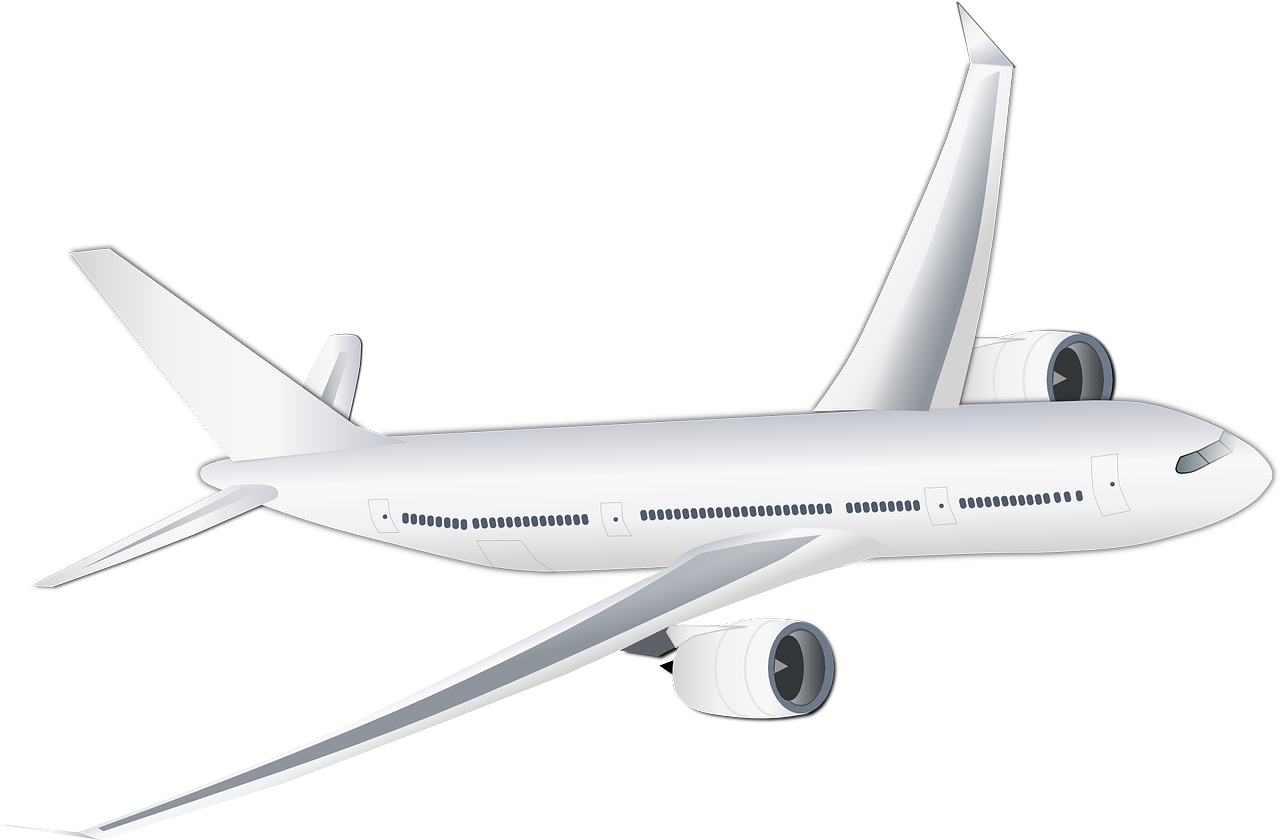
\includegraphics[width=\textwidth]{img/airplane.png}}; \\
\node(s2){
\includegraphics[width=\textwidth]{img/woman.png}};       \& \& \& \node(c2) {
\includegraphics[width=2\textwidth]{img/logistics.png}}; \\
\node(s3){
\includegraphics[width=\textwidth]{img/man.png}};         \& \& \& \node(c3) {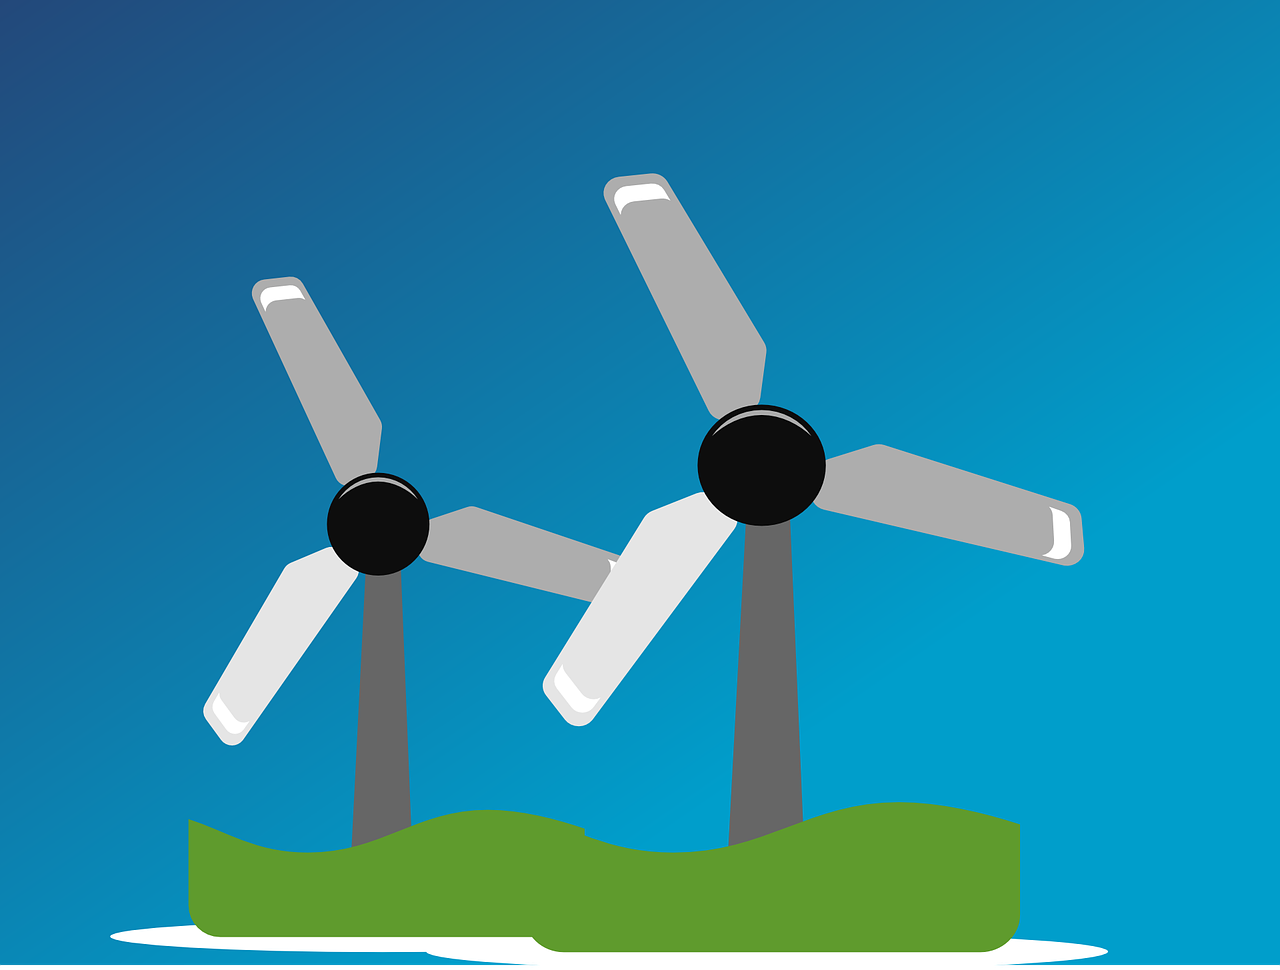
\includegraphics[width=2\textwidth]{img/enrgy.png}}; \\
\node[defaultStyle, draw, onslide={<3->{highlight2}}](s4){
\includegraphics[width=\textwidth]{img/woman2.png}};      \& \\
};

\draw[onslide={<2->{highlight}}] (s1) -- (c1);
\draw[] (s1) -- (c2);

\draw[onslide={<2->{highlight}}] (s2) -- (c1);
\draw[] (s2) -- (c3);

\draw[onslide={<2->{highlight}}] (s3) -- (c2);

\draw[onslide={<2->{highlight}}] (s4) -- (c3);
\draw[] (s4) -- (c2);
%
%\draw[onslide={<1-2>{highlight}}] (z) -- (3);
%\draw[onslide={<3>{highlight}}] (z) -- (2);
%
%\draw[onslide={<1-2>{highlight}}] (t) -- (2);
%\draw[] (t) -- (1);
%\draw[onslide={<3>{highlight}}] (t) -- (5);
%\draw[] (t) -- (3);
%\draw[] (t) -- (4);
%\draw[onslide={<1>{highlight}}] (u) -- (4);
%\draw[] (u) -- (3);
%\draw[] (u) -- (5);
%\draw[] (u) -- (6);
\end{tikzpicture}
\end{center}
\onslide<2->{This \alert{assignment} respects students' preferences (edges) \onslide<3->{but ignores {\color{CornflowerBlue} companies' preferences}.}}
%\onslide<4->{\tiny OK, es ist nicht wirklich ein \emph{Matching} da Firmen mehr als einen Studenten betreuen \ldots }
\end{frame}

\begin{frame}[fragile]{Mentor Matching: Constraint Model}
\begin{lstlisting}
int: n; set of int: STUDENT = 1..n;
int: m; set of int: COMPANY = 1..m;

% assign students to companies
array[STUDENT] of var COMPANY: worksAt;


int: minPerCompany = 1; int: maxPerCompany = 3;
constraint global_cardinality_low_up ( 
           worksAt, [c | c in COMPANY], 
           [minPerCompany | c in COMPANY], 
           [maxPerCompany | c in COMPANY]); 
           
solve 
search pvs_BAB();
\end{lstlisting}
\end{frame}

\begin{frame}[fragile]{Mentor Matching: FAS* Instance}
\begin{lstlisting}
% fas2016.mzn

n = 5; % students
m = 3; % companies

% student names for better readability 
int: britney = 1;
int: christina = 2;
int: drdre = 3; 
int: eminem = 4; 
int: falco = 5; 

% company names 
int: disney = 1;
int: warner = 2;
int: uniaugsburg = 3;
\end{lstlisting}

\end{frame}

\begin{frame}[fragile]{Mentor Matching: Preferences}
\begin{lstlisting}
PVS: students = new ConstraintRelationships("students") {
   soft-constraint britneyDisney : 'worksAt[britney] = disney';
   soft-constraint britneyWarner : 'worksAt[britney] = warner';
   soft-constraint eminemUnia : 'worksAt[eminem] = uniaugsburg';
   crEdges : '[|  mbr.britneyDisney , mbr.britneyWarner | mbr.eminemUnia, mbr.britneyDisney |]';
   useSPD: 'true' ;
}; 

PVS: companies = new ConstraintRelationships("companies") {
   soft-constraint disneyChristina : 'worksAt[christina] = disney';
   soft-constraint disneyFalco : 'worksAt[falco] = disney';
   soft-constraint uniaugsburg : 'worksAt[britney] = uniaugsburg';
   
   crEdges : '[| mbr.disneyFalco, mbr.uniaugsburg |]';
   useSPD: 'true' ;
}; 
\end{lstlisting}
\end{frame}

\begin{frame}[fragile]{Mentor Matching: Behavior I}
\begin{lstlisting}
solve ToWeighted(students) lex ToWeighted(companies);
\end{lstlisting}
\begin{Verbatim}[fontsize=\small]
Intermediate solution:worksAt = [3, 2, 1, 1, 1]
Valuations: penCompanies = 1; penStudents = 6
----------
Intermediate solution:worksAt = [2, 3, 1, 1, 1]
Valuations: penCompanies = 3; penStudents = 3
----------
Intermediate solution:worksAt = [1, 1, 2, 3, 1]
Valuations: penCompanies = 2; penStudents = 3
----------
Intermediate solution:worksAt = [2, 1, 1, 3, 1]
Valuations: penCompanies = 2; penStudents = 2
----------
==========
\end{Verbatim}

\end{frame}

\begin{frame}[fragile]{Mentor Matching: Behavior II}
\begin{lstlisting}
solve ToWeighted(companies) lex ToWeighted(students);
\end{lstlisting}
\begin{Verbatim}[fontsize=\small]
Intermediate solution:worksAt = [3, 2, 1, 1, 1]
Valuations: penCompanies = 1; penStudents = 6
----------
Intermediate solution:worksAt = [3, 1, 2, 1, 1]
Valuations: penCompanies = 0; penStudents = 6
----------
Intermediate solution:worksAt = [3, 1, 2, 3, 1]
Valuations: penCompanies = 0; penStudents = 5
----------
==========
\end{Verbatim}

\end{frame}


\begin{frame}[fragile]{Mentor Matching: Winter Term 15/16}
\begin{itemize}
\item Collected preferences from emails 

\begin{parchment}
\begin{verbatim}
"the favorites":
1. JuneDied-Lynx- HumanIT
2. Cupgainini
 
"I could live with that":
3. Seamless-German
4. gsm systems
5. Yiehlke
 
"I think, we won't be happy":
6. APS
7. Delphi Databases
\end{verbatim} 
\end{parchment}
\end{itemize}
\end{frame}

\begin{frame}[fragile]{Mentor Matching: Winter Term 15/16}
\begin{itemize}
\item Priority for \alert{students}
\begin{itemize}
\item[-] What are companies supposed to do with unhappy students?
\end{itemize}
\item Search space: 7 Companies for 16 students $\rightarrow 7^{16} = 3.3233 \cdot 10^{13}$
\vspace*{2ex}
\item Led to a constraint problem with
\begin{itemize}
\item[-] 77 students' preferences (soft constraints) of 16 students
\item[-] in total 114 soft constraints (37 company preferences) 
\end{itemize}

\vspace*{2ex}

\item \emph{Proven} optimal solution
\begin{itemize}
\item[-] 6 minutes 
\end{itemize}
\end{itemize}
\end{frame}


\begin{frame}{Evaluationsergebnisse}

\end{frame}

\begin{frame}{Kooperationen}
\begin{itemize}
\item[] \alert{Konzepte, Sprachdesign MiniBrass}
\begin{itemize}
\item[-] AS, Alexander Knapp, Gerrit Anders, Oliver Kosak
\end{itemize}
\item[] \alert{Anwendungen, Multiagenten-Einsatz}
\begin{itemize}
\item[-] Alexander Schubert (MSc-Thesis: Einsatz von Voting-Verfahren), Markus Tolls (MSc-Thesis: Formalisierung von Task-Allocation-Problemen)
\end{itemize}
\end{itemize}
\end{frame}

\begin{frame}{Outreach}
\begin{itemize}
\item Vortrag Helmholtz-Zentrum München
\item Vortrag FH Hagenberg
\item Tutorial @ SASO 2016
\end{itemize}
\end{frame}



\begin{frame}[allowframebreaks]
        \frametitle{References}
        \bibliographystyle{apalike}
        \bibliography{../common}
\end{frame}


\end{document}

